\subsection{MFT}
\label{MFT:datarate}

The MFT is a Silicon tracker which will be installed in the muon spectrometer acceptance. It is composed of 6 planes of Silicon pixel sensors. A version with 5 planes was considered in the LoI Addendum. It has been decided to add a sixth plane for redundancy in the tracking. 
A description of the detector can be found in the ALICE LoI addendum~\cite{LOI_Addendum}.
In order to cover the full area, 668 ladders of 1 to 5 sensors with a total of 2530 sensors are necessary.

Three main components are contributing to the hit rate of the MFT: the Pb--Pb collision itself, the hits induced by the QED processes (mainly low $p_{T}$ electrons at low angles) and the noisy pixels.

Table~\ref{tab:MFTrate} summarizes the number of hits  in the MFT expected in the following conditions: continuous readout with
16~\ums frames at 100~kHz \pbpb collisions and 
a random noise at the rate of $10^{-5}$ per pixel. Minimum bias collision multiplicity is assumed to be one third of that in the central collision.


\begin{table}[ht]
\centering
\begin{tabular}{ | c | c | c | c | c |}
%\begin{tabular}{ | l | l | l | l | l | l | }
\hline
\multirow{2}{*}{Plane}   & Single central  & Min.bias \pbpb  &  QED & \multirow{2}{*}{Noisy Pixels} \\ 
    &  \pbpb collision &  16 \ums @ 100 kHz &  16 \ums @ 100 kHz & \\ \hline
0   & 3480           & 3016                & 1424     &     763       \\ \hline
1   & 3480           & 3016                & 1424     &      763      \\ \hline
2  & 3950           & 3423                & 1512      &       926    \\ \hline
3  & 3910           & 3389                &  1403       &      1090    \\ \hline
4  & 3820           & 3311                 &  1274        &      1205   \\ \hline
5  & 4100           & 3553                  &  1271         &     1325   \\ \hline
\multicolumn{2}{|c|}{Total hit clusters }                  & \multirow{2}{*}{19708}     &   \multirow{2}{*}{8308}     &   \multirow{2}{*}{6072}       \\ 
\multicolumn{2}{|c|}{per 16 \ums frame}                  &     &     &       \\ \hline
\end{tabular}
\caption{Hit rates from hadronic collisions and QED electrons. Random noise rate assumed to be $10^{-5}$ per pixel per 16~\ums 
readout frame.}
\label{tab:MFTrate}
\end{table}

Two kinds of clusters can be distinguished: single-pixel clusters which the primary source is noisy pixel and the multi-pixel clusters induced by particle crossing the detector. 
The clusters are assumed to be encoded into 40 bits per cluster.
The total data flow output is then estimated to be 10.1~GB/s for the entire MFT.
The data rate reduces to 7.2~GB/s when assuming a 50~kHz minimum bais \pbpb collision rate still with a 16~\ums readout time per frame.
With such raw data flow rate, an online clusterization is mandatory to reduce the amount of data written on tape (see section~\ref{sec:MFTClusterization}).

The local on-detector readout is proposed to be performed by GigaBit Transceiver (GBT) versatile link developed at CERN which will act as a data concentrator.
Fig.~\ref{fig:mft:schematic} presents a schematic of the readout scheme.
A total of 166 GBT links are foreseen to  handle the data flow.

\begin{figure}[h]
\centering
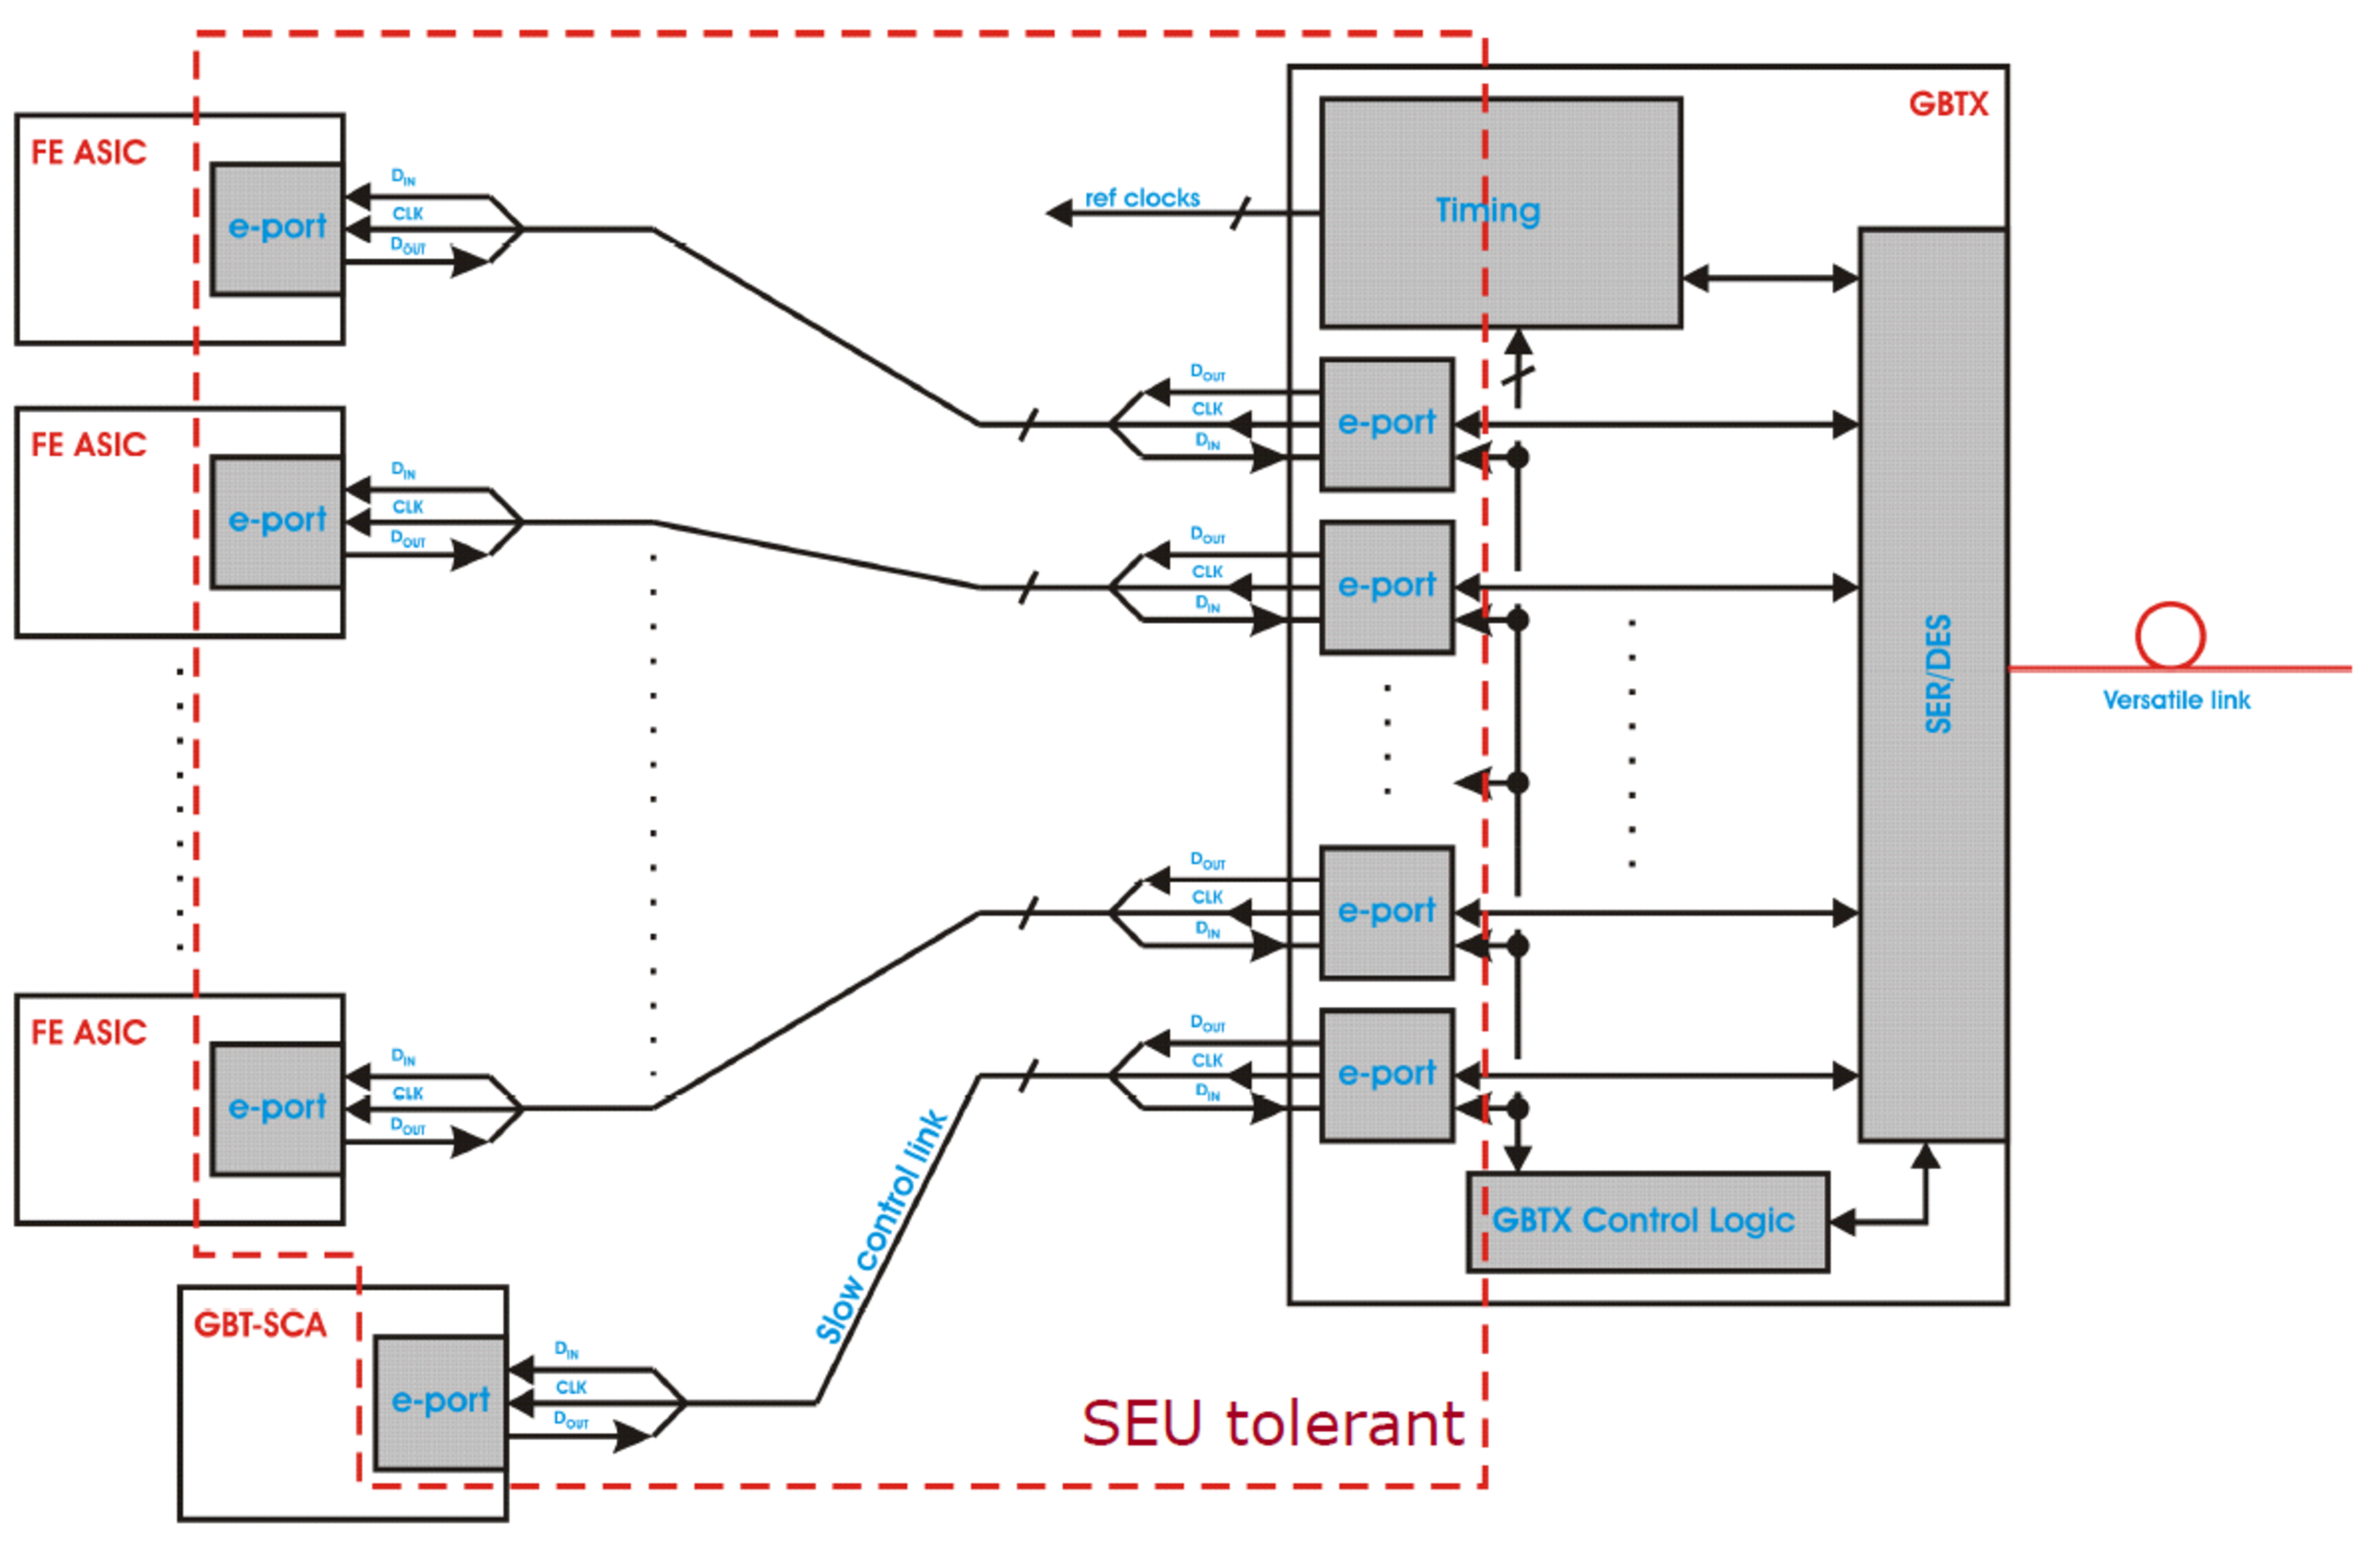
\includegraphics[width=0.9\textwidth]{MFT/Schematic.pdf}
\caption{\label{fig:mft:schematic} 
Possible schematic of the on-detector readout of the MFT using GBT as a concentrator.}
\end{figure}

